Para la realización de este trabajo se ha utilizado tres conjuntos de datos. Cada conjunto de datos se ha creado aleatoriamente utilizando la herramienta \href{https://www.generatedata.com/}{generatedata.com} y se ha guardado en un fichero \textit{CSV}. Los ficheros \textit{CSV} contienen información que representan parejas de nodos (vértices), con pesos en las aristas que forman un grafo no dirigido.

El primer conjunto de datos lo forma el grafo de la figura \ref{grafo_1}. Se ha utilizado para describir sobre los ejemplos de los diferentes algoritmos. 

\renewcommand{\figurename}{Figura}
\begin{figure}[h]
	\centering
	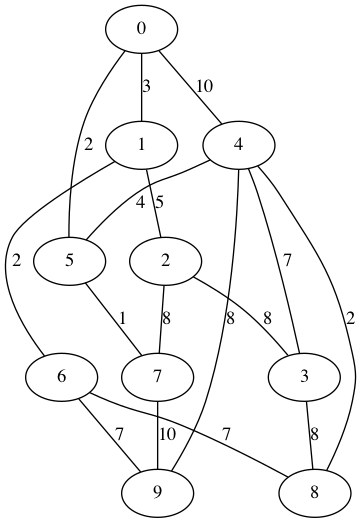
\includegraphics[scale=0.4]{../dataset/dataset}
	\vspace{1mm}
	\caption{Grafo no dirigido de 10 nodos}
	\label{grafo_1}
\end{figure}


El segundo conjunto de datos lo forma el grafo de la figura \ref{grafo_2}

\begin{figure}[h]
	\centering
	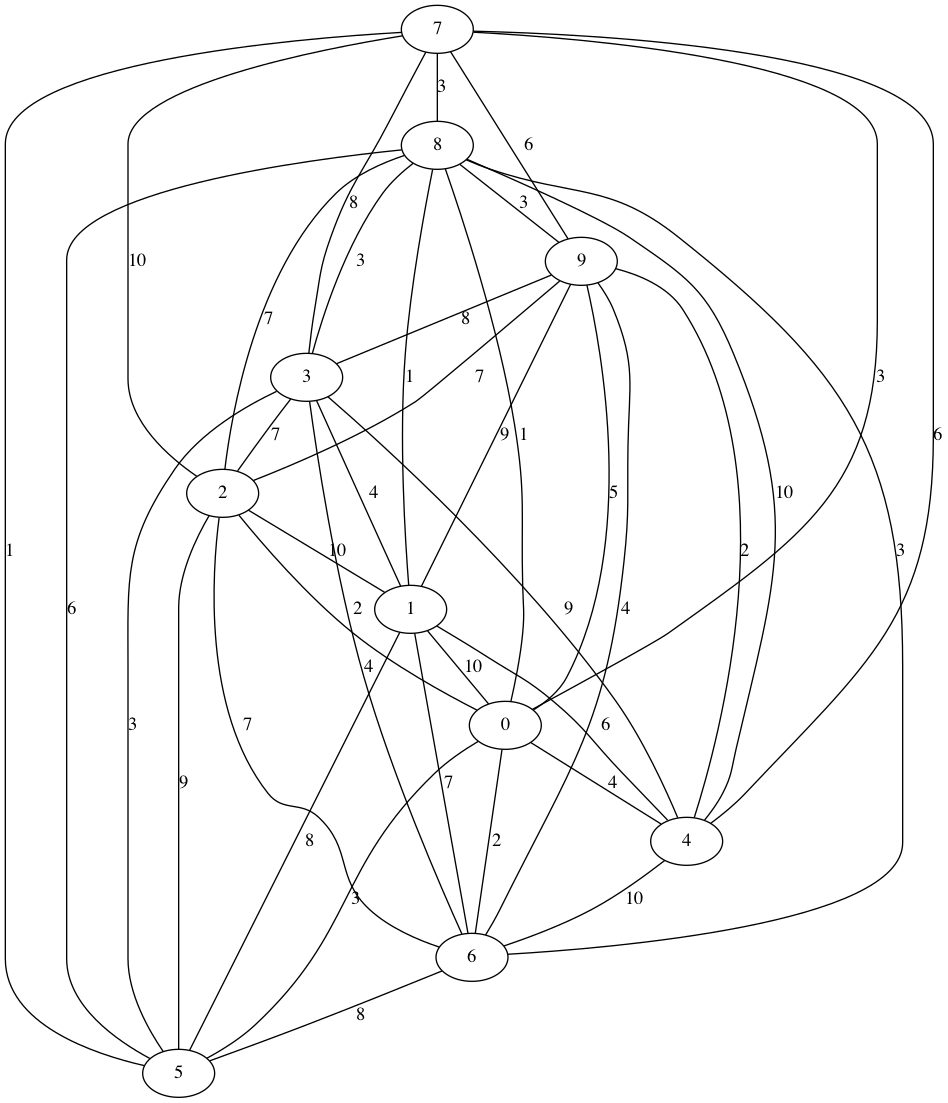
\includegraphics[scale=0.3]{../dataset/90_10_dataset}
	\vspace{1mm}
	\caption{Grafo no dirigido de 10 nodos}
	\label{grafo_2}
\end{figure}

El tercer conjunto de datos lo forma el grafo de la figura \ref{grafo_3}.

\begin{figure}[h]
	\centering
	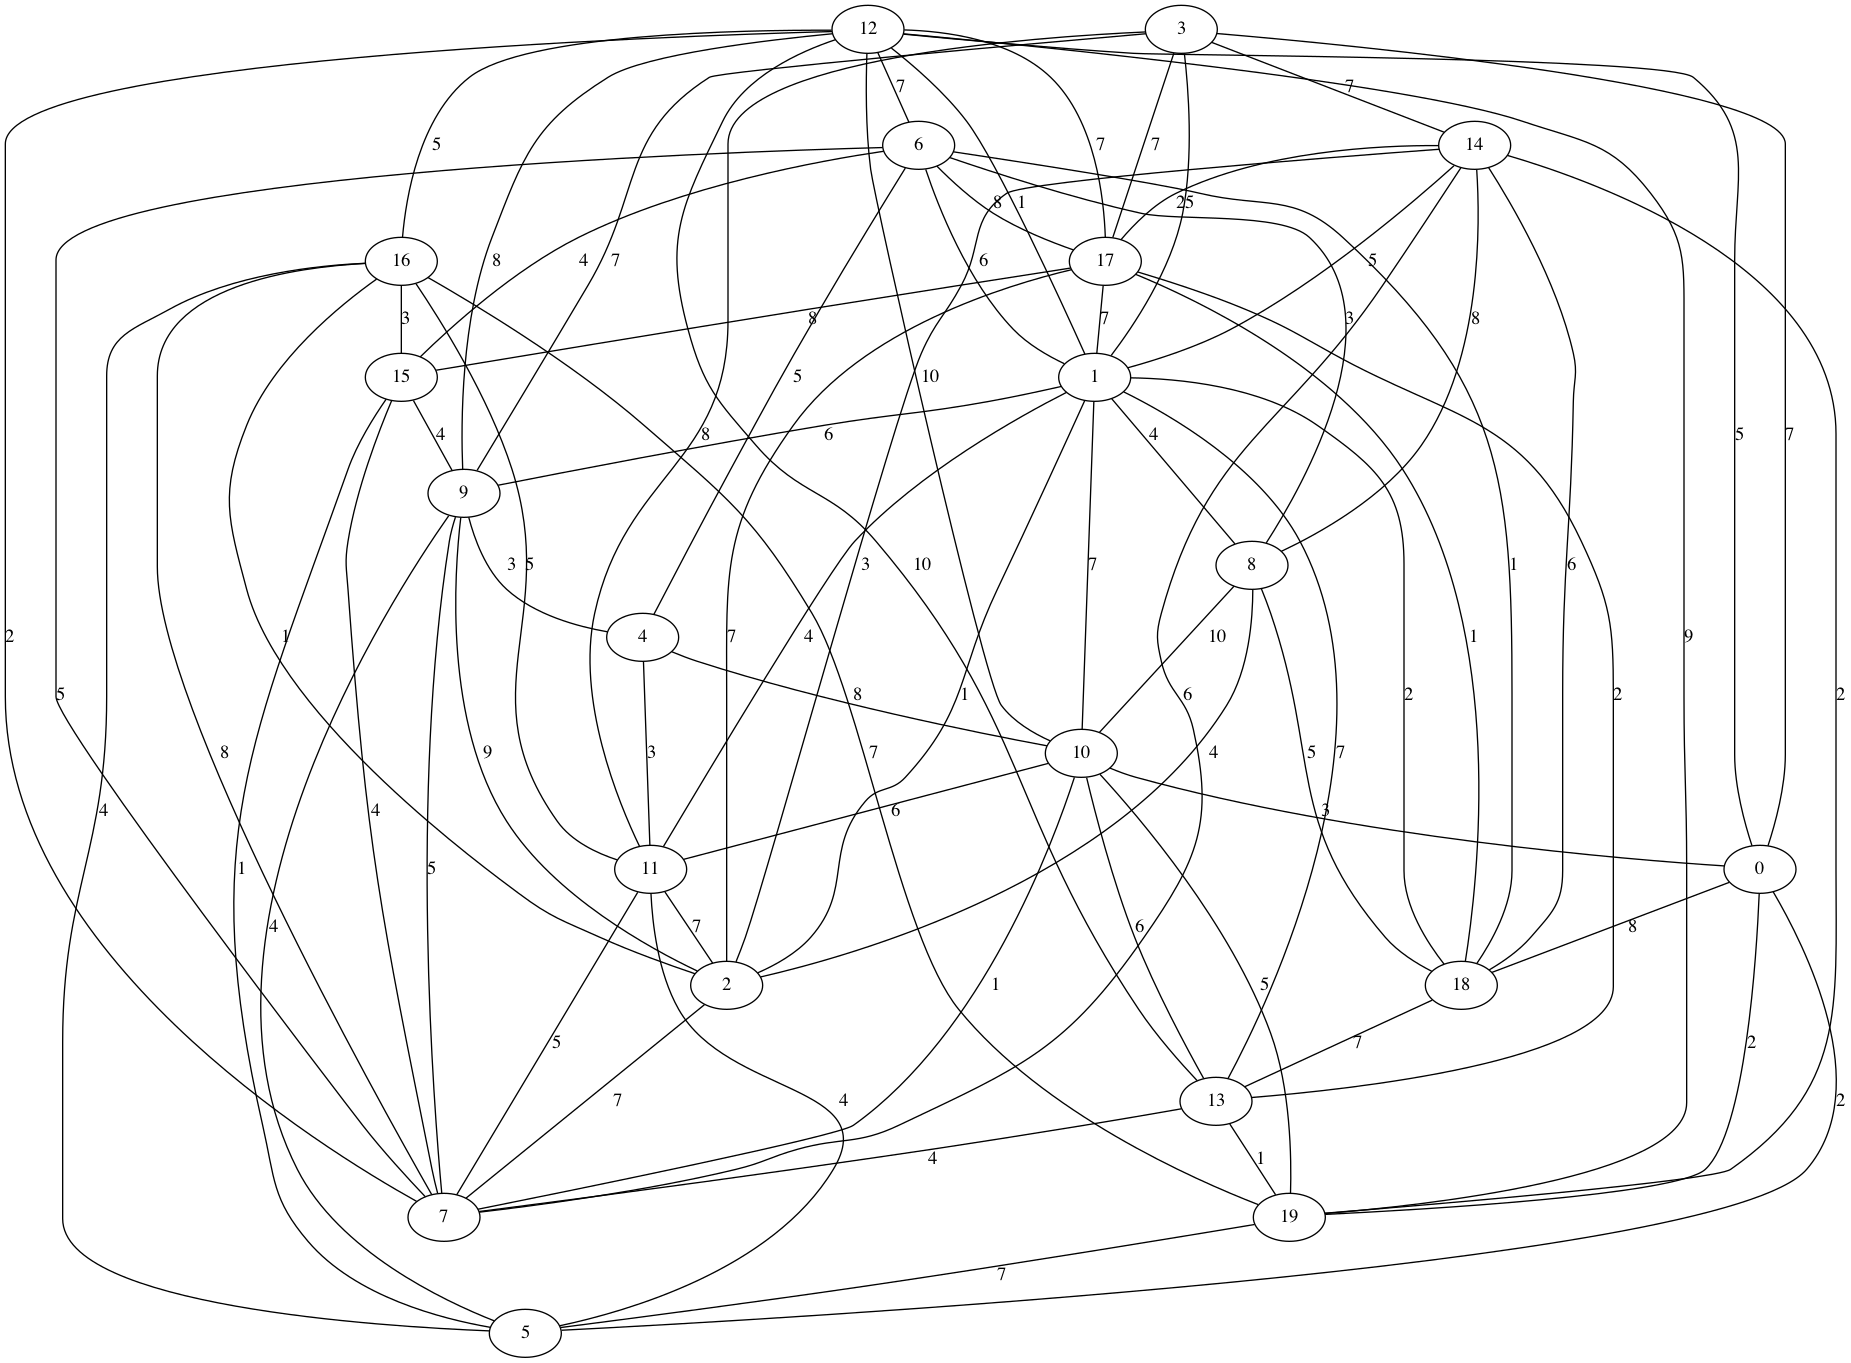
\includegraphics[scale=0.2]{../dataset/95_20_dataset}
	\vspace{1mm}
	\caption{Grafo no dirigido de 20 nodos}
	\label{grafo_3}
\end{figure}

El segundo y tercer conjunto de datos se han utilizado para la comparativa entre los diferentes algoritmos.

